\documentclass[11pt,portuguese]{fphw}
	\usepackage[utf8]{inputenc}
	\usepackage{algorithm2e}
	\usepackage{mathtools}
	\usepackage{amssymb}
	\usepackage{tikz}
	\usepackage{upgreek}
	\usetikzlibrary{automata}
	
	\title{Prova \#2}
	\author{André Luiz Cavalcante Ferreira de Souza}
	\date{11 de fevereiro, 2020}
	\class{Linguagens Formais e Autômatos}
	\professor{Julliano Rosa}
	\institute{Instituto de Informática - Universidade Federal de Goiás}
	\begin{document}
		\maketitle
		
		\section*{Exercício 1}
		\begin{problem}
			\textbf{1) }Seja a gramática $G = ( \{0, 1\}, \{S, A\}, S, P\} )$, com o conjunto de produções \textit{P} abaixo:
			
			$$
			P = 
			\begin{dcases}
				\begin{rcases}
				 S \rightarrow SAS \mid 0,
				 \\
				 A \rightarrow ASA \mid 1
				 \end{rcases}
			\end{dcases}
			$$
			\linebreak
			Mostre que \textit{G} é ambígua.
		\end{problem}
			\subsection*{Solução}
				Considere \textit{s} = 0101010. Desta forma, podemos construir a seguinte
				derivação:
				
				\begin{itemize}
					\item
						\begin{equation*}
						S \Rightarrow SAS \Rightarrow 0AS \Rightarrow 01S \Rightarrow
						01SAS 
						\Rightarrow 010AS \Rightarrow 0101S \Rightarrow 0101SAS 
						\Rightarrow 01010AS \Rightarrow 010101S 
						\Rightarrow 0101010.
						\end{equation*}
						
					\item$
						S \Rightarrow SAS \Rightarrow SASAS \Rightarrow SASASAS
						\Rightarrow 0ASASAS \Rightarrow 01SASAS \Rightarrow 010ASAS 
						\Rightarrow 0101SAS \Rightarrow 01010AS \Rightarrow 010101S 
						\Rightarrow 0101010.
					$
				\end{itemize}
				
				Portanto, concluímos que a gramática é ambígua, pois existem duas árvores
				de derivação à esquerda.
			
		\section*{Exercício 2}
			\begin{problem}
				\textbf{2) }Converta para forma normal de Chomsky a gramática livre de contexto 
				especificada pelo conjunto de regras de derivação a  seguir. Mostre as 						regras
				de derivação obtidas em cada passo intermediário especificando a 
				transformação utilizada.
				\linebreak
				$$
					P = \begin{dcases}
						\begin{rcases}
						A \rightarrow BAB \mid B \mid \varepsilon,\\
						B \rightarrow 00 \mid \varepsilon
						\end{rcases}
					\end{dcases}
				$$
			\end{problem}
			\subsection*{Resposta}
				A resposta é bem trivial, veja só!
				\newcommand{\barra}{\mid}
				\begin{enumerate}
					\item Removendo recursão em \textit{A}:
					$$
						P = \begin{dcases}
						\begin{rcases}
							A \rightarrow A',\\
							A' \rightarrow BA'B \barra B \barra \varepsilon,\\
							B \rightarrow 00 \mid \varepsilon
							\end{rcases}
						\end{dcases}
					$$
					\item Removendo transição $\varepsilon$ em 								\textit{B}:
						$$
						P = \begin{dcases}
						\begin{rcases}
							A \rightarrow A',\\
							A' \rightarrow BA'B \barra B \barra \varepsilon
							 \barra BA' \barra A'B \barra A',\\
							B \rightarrow 00
							\end{rcases}
						\end{dcases}
					$$
					\newpage
					\item Removendo transição $\varepsilon$ em
						\textit{A}' e removendo recursão desnecessária:
						$$
						P = \begin{dcases}
						\begin{rcases}
							A \rightarrow A' \barra \varepsilon,\\
							A' \rightarrow BA'B \barra B 
							 \barra BA' \barra A'B,\\
							B \rightarrow 00
							\end{rcases}
						\end{dcases}
						$$
					\item Criando nova regra $ X \rightarrow 0$
					e substituindo ocorrências unitárias de \textit{B}:
						$$
						P = \begin{dcases}
						\begin{rcases}
							A \rightarrow A' \barra \varepsilon,\\
							A' \rightarrow BA'B \barra XX 
							 \barra BA' \barra A'B,\\
							B \rightarrow XX,\\
							X \rightarrow 0
							\end{rcases}
						\end{dcases}
						$$
					\item Criando regra para \begin{math}A'B\end{math} e substituindo
					suas ocorrências:
						$$
						P = \begin{dcases}
						\begin{rcases}
							A \rightarrow A' \barra \varepsilon,\\
							A' \rightarrow BY \barra XX 
							 \barra BA' \barra A'B,\\
							B \rightarrow XX,\\
							X \rightarrow 0,\\
							Y \rightarrow A'B
							\end{rcases}
						\end{dcases}
						$$
					\item Substituindo regra unitária \textit{A}:
						$$
						P = \begin{dcases}
						\begin{rcases}
							A \rightarrow BY \barra XX 
							 \barra BA' \barra A'B \barra \varepsilon,\\
							A' \rightarrow BY \barra XX 
							 \barra BA' \barra A'B,\\
							B \rightarrow XX,\\
							X \rightarrow 0,\\
							Y \rightarrow A'B
							\end{rcases}
						\end{dcases}
						$$
				\end{enumerate}
				Desta forma, concluimos obtendo uma gramática na Forma Normal de Chomsky.
					
				\section*{Exercício 3}
					\begin{problem}
						Construa um PDA que aceite a linguagem \textit{L} = \{
						\begin{math}
							a^i b^i c^j \mid i,j \geq 0
						\end{math}
						\}.
					\end{problem}
					\subsection*{Resposta} Começemos criando uma gramática \textit{G}
					que gera a linguagem:
						\begin{enumerate}%%or itemize
						\item Gramática:
						\[
							P = \begin{dcases}
								\begin{rcases}
									S \rightarrow AB \mid \varepsilon,\\
									A \rightarrow aAb \mid \varepsilon,\\
									B \rightarrow cB \mid \varepsilon
								\end{rcases}
							\end{dcases}
						\]
						\newpage
						\item Autômato:
							\\
							\\
							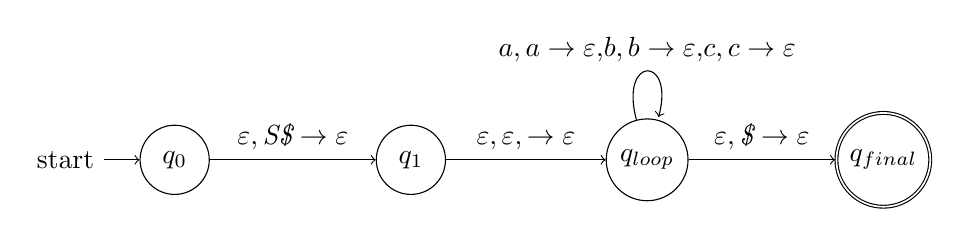
\begin{tikzpicture}[->, node distance=3cm]
								\node[initial, state](A){$q_0$};
								\node[state](B)[right of=A]{$q_1$};
								\node[state](C)[right of=B]{$q_{loop}$};
								\node[accepting, state](D)[right of=C]{$q_{final}$};
								
								\path (A) edge[above] node{$\varepsilon, \textit
								{S\$} \rightarrow \varepsilon$}(B);
								
								\path (B) edge[above] node{$\varepsilon, \varepsilon,
								\rightarrow \varepsilon$}(C);
								
								\path (C) edge[loop above] node{
								$a, a \rightarrow \varepsilon$,\linebreak
								$b, b \rightarrow \varepsilon$,\\
								$c, c \rightarrow \varepsilon$\\
								}(C);
								\path(C) edge[above] node{$\varepsilon, \textit{\$}
								 \rightarrow \varepsilon$}(D);
								
							\end{tikzpicture}
						\end{enumerate}
		\section*{Exercicio 4}
			\begin{problem}
				Sejam $\Sigma = \{a, b, \# ,\}$ e $L \in \Sigma^*$ definida a seguir:
				$$L = \{w\#t \mid w \subseteq t \wedge t, w \in \{a,b\}^*\}$$
				
				Prove que \textit{L} não é livre de contexto.
			\end{problem}
			\subsection*{Resposta}
				Esta é a resposta:

	\end{document}